\documentclass{article}
\providecommand{\versionnumber}{1.0.0}
\usepackage[utf8]{inputenc}
\usepackage[includeheadfoot, margin=1em,headheight=2em]{geometry}
\usepackage{titling}
\usepackage{hyperref}
\usepackage[italian]{babel}
\geometry{a4paper, left=2cm, right=2cm, top=2cm, bottom=2cm}
\usepackage{graphicx}
\usepackage{float}
\usepackage{enumitem}
\usepackage{array}
\usepackage{eurosym}
\newcolumntype{P}[1]{>{\centering\arraybackslash}p{#1}}
\renewcommand{\arraystretch}{1.5} % Default value: 1
\setlength{\droptitle}{-6em}
\usepackage{capt-of}

%font
\usepackage[defaultfam,tabular,lining]{montserrat}
\usepackage[T1]{fontenc}
\renewcommand*\oldstylenums[1]{{\fontfamily{Montserrat-TOsF}\selectfont #1}}

%custom bold 
\usepackage[outline]{contour}
\usepackage{xcolor}
\newcommand{\custombold}{\contour{black}}

%table colors
\usepackage{color, colortbl}
\definecolor{Blue}{rgb}{0.51,0.68,0.79}
\definecolor{LightBlue}{rgb}{0.82,0.87,0.90}
\definecolor{LighterBlue}{rgb}{0.93,0.95,0.96}

%Header
\usepackage{fancyhdr, xcolor}
\pagestyle{fancy}
\let\oldheadrule\headrule% Copy \headrule into \oldheadrule
\renewcommand{\headrule}{\color{Blue}\oldheadrule}% Add colour to \headrule
\renewcommand{\headrulewidth}{0.2em}
\fancyhead[L]{Piano di progetto}
\fancyhead[C]{Cybersorceres}
\fancyhead[R]{versione \versionnumber}

\title{\Huge{\textbf{Piano di progetto}}\vspace{-1em}}
\author{CyberSorcerers Team}
\date{}
\begin{document}
\maketitle
\vspace{-3em}
\begin{figure}[h]
  \centering
  
\includegraphics[width=6cm, height=6cm]{documenti/logo rotondo.png}
  \label{fig:immagine}
\end{figure}

\vspace{3em}
\large{
\begin{center}
    \begin{tabular}{P{24em}}
        \rowcolor{Blue}
        \textbf{Membri del team:}\\
        \rowcolor{LighterBlue}
        \custombold{Sabrina Caniato}\\
        \rowcolor{LightBlue}
        \custombold{Giulia Dentone}\\
        \rowcolor{LighterBlue}
        \custombold{Nicola Lazzarin}\\
        \rowcolor{LightBlue}
        \custombold{Giovanni Moretti}\\
        \rowcolor{LighterBlue}
        \custombold{Andrea Rezzi}\\
        \rowcolor{LightBlue}
        \custombold{Samuele Vignotto}\\
    \end{tabular}
\end{center}}
\newpage
\textbf{Registro dei Cambiamenti - Changelog}
\begin{center}
\begin{tabular}{P{5em} P{6em} P{8em} P{8em} P{10em}} 
  \rowcolor{Blue}
    \custombold{Versione} & \custombold{Data} & \custombold{Autore} &
    \custombold{ Verificatore} & \custombold{Dettaglio}\\
    \rowcolor{LightBlue}
     1.0.1 & 5/04/2024 & Nicola Lazzarin & Giulia Dentone & Correzione grafici\\
    \rowcolor{LighterBlue}
     1.0.0 & 1/03/2024 & Nicola Lazzarin & Samuele Vigonotto & Update dei diagrammi di Gantt\\
    \rowcolor{LightBlue}
     0.5.0 & 20/01/2024 & Giulia Dentone & Nicola Lazzarin & Aggiunta della mitigazione dei rischi\\
    \rowcolor{LighterBlue}
     0.4.2 & 17/01/2024 & Samuele Vignotto & Andrea Rezzi & Update del consuntivo\\
    \rowcolor{LightBlue}
     0.4.1 & 13/01/2024 & Sabrina Caniato & Giulia Dentone & Update del consuntivo\\
    \rowcolor{LighterBlue}
     0.4.0 & 12/01/2024 & Samuele Vignotto & Giovanni Moretti & Compilazione del consuntivo\\
    \rowcolor{LightBlue}
     0.3.3 & 07/01/2024 & Nicola Lazzarin & Sabrina Caniato & Inserimento delle caption delle immagini\\
    \rowcolor{LighterBlue}
     0.3.2 & 03/01/2024 & Andrea Rezzi & Nicola Lazzarin & Update dei riepiloghi\\ 
    \rowcolor{LightBlue}
    0.3.1 & 03/01/2024 & Giovanni Moretti & Sabrina Caniato & Update dei riepiloghi\\
    \rowcolor{LighterBlue}
     0.3.0 & 27/12/2023 & Samuele Vignotto & Giovanni Moretti & Update della sezione preventivo con i riepiloghi\\ 
    \rowcolor{LighterBlue}
     0.2.1 & 19/12/2023 & Samuele Vignotto & Giulia Dentone & Aggiunta sezioni e contenuto sezione "Periodi" della sezione "Pianificazione"\\
    \rowcolor{LightBlue}
     0.2.0 & 18/12/2023 & Giulia Dentone & Nicola Lazzarin & Compilazione della sezione Pianificazione con descrizione fasi e periodi.\\
    \rowcolor{LighterBlue}
     0.1.1 & 16/12/2023 & Giovanni Moretti & Sabrina Caniato & Update della sezione dei rischi\\
\end{tabular}
\end{center}

\begin{center}
\begin{tabular}{P{5em} P{6em} P{8em} P{8em} P{10em}} 
    \rowcolor{LightBlue}
    0.1.0 & 15/12/2023 & Sabrina Caniato & Giovanni Moretti & Aggiunta della sezione dei rischi\\
    \rowcolor{LighterBlue}
     0.0.1 & 14/12/2023 & Andrea Rezzi & Nicola Lazzarin & efinizione struttura del documento e scheletro delle sezioni. Scrittura introduzione ed obiettivi delle diverse sezioni\\ 
\end{tabular}
\end{center}
\newpage
\tableofcontents
\newpage
\section{Introduzione}
\subsection{Scopo del documento}
Lo scopo del documento è quello di normare il processo di sviluppo del progetto, in tempi e modalità. In particolare viene effettuata un'analisi dei rischi, e delle relative azioni e modalità che verranno adottate per mitigarli. Il documento viene redatto con un approccio incrementale, al fine di poter implementare modifiche concordate dal gruppo o dal proponente.

\subsection{Obiettivo del prodotto}
Prima di poter procedere all'analisi dei rischi, è necessario identificare chiaramente l'obiettivo del prodotto: la creazione di una web app che, tramite l’uso di IA\textsubscript{G}(ChatGPT4 e Bedrock) crei, a partire dalle richieste del cliente, epic user stories\textsubscript{G} e confrontarle con il codice sviluppato. Il fine è quello di informare il cliente dello stato di avanzamento dello sviluppo del prodotto e rendere possibile al Project Manager\textsubscript{G} e al cliente rilasciare dei
feedback (riguardanti, in base all'utente utilizzatore, l'adeguatezza delle stories\textsubscript{G} o il prodotto finale) al fine di migliorare l’IA\textsubscript{G}. In ultimo è richiesto un confronto tra le IA\textsubscript{G} utilizzate e lo sviluppo di un plugin utile agli sviluppatori e al Project Manager\textsubscript{G}.

\subsection{Glossario}
I termini impiegati in questo testo potrebbero suscitare incertezze circa il loro significato, rendendo quindi necessaria una definizione per evitare ambiguità. Tali termini sono identificati da una lettera "G" maiuscola posta in pedice alla parola, e la loro spiegazione è fornita nel Glossario v1.0.0.

\subsection{Riferimenti}
\textbf{Riferimenti normativi}
\begin{itemize}
        \item \href{https://www.math.unipd.it/~tullio/IS-1/2023/Progetto/C7.pdf}{C7.pdf}
        \item{Norme di progetto}
\end{itemize}
\textbf{Riferimenti informativi}
\begin{itemize}
        \item Argomento T2 - Processi di ciclo di vita
        \item Argomento T4 - Gestione di progetto
\end{itemize}

\section{Analisi dei rischi}
Questa sezione si occupa di analizzare le difficoltà riscontrabili dal proponente ed evitare problemi che possono intercorrere tra lo stato di avanzamento e il completamento del progetto. Analizzeremo dunque ciascun rischio, descrivendolo e giudicando il suo grado di rischio, pericolosità, precauzione e le misure di mitigazione adottate. Il fine è quello di permettere una loro facile identificazione e un continuo monitoraggio. Abbiamo deciso di suddividerli secondo tre differenti categorie:le difficoltà personali, le difficoltà organizzative interne ed esterne e le difficoltà tecnologiche/software.

\subsection{Rischi organizzativi}
\subsubsection{Comunicazione interna}
\begin{center}
\begin{tabular}{P{10em} P{20em}} 
    \rowcolor{LighterBlue}
     Descrizione & Mancata reperibilità sincrona dei membri del gruppo, data da eventuali impegni personali.\\ 
    \rowcolor{LightBlue}
    Occorrenza & Media\\
    \rowcolor{LighterBlue}
    Pericolosità & Alta \\
    \rowcolor{LightBlue}
    Precauzioni & Ogni membro del gruppo comunica vocalmente i propri impegni straordinari della settimana ad ogni riunione interna. \\
    \rowcolor{LighterBlue}
    Misure di contenimento & Ogni membro del gruppo compilerà un documento Drive interno  con i suoi impegni fissi o inderogabili. \\
\end{tabular}
\captionof{table}{Rischi della comunicazione interna}
\label{tab:cominterna}
\end{center}

\subsubsection{Comunicazione esterna}
\begin{center}
\begin{tabular}{P{10em} P{20em}} 
    \rowcolor{LighterBlue}
     Descrizione & Difficoltà nella comunicazione repentina con l'azienda.\\ 
    \rowcolor{LightBlue}
    Occorrenza & Bassa\\
    \rowcolor{LighterBlue}
    Pericolosità & Alta \\
    \rowcolor{LightBlue}
    Precauzioni & Richiedere al cliente il modo più semplice e celere di ottenere una sua risposta. \\
    \rowcolor{LighterBlue}
    Misure di contenimento & Creazione di un canale Slack attivo.\\
\end{tabular}
\captionof{table}{Rischi della comunicazione esterna}
\label{tab:comesterna}
\end{center}

\subsubsection{Mancata esperienza professionale}
\begin{center}
\begin{tabular}{P{10em} P{20em}} 
    \rowcolor{LighterBlue}
     Descrizione & Gran parte dei i membri del gruppo non ha esperienze significative in ambito di sviluppo o professionali.\\ 
    \rowcolor{LightBlue}
    Occorrenza & Alta\\
    \rowcolor{LighterBlue}
    Pericolosità & Media \\
    \rowcolor{LightBlue}
    Precauzioni & Ogni membro deve essere trasparente nel comunicare le sue competenze. \\
    \rowcolor{LighterBlue}
    Misure di contenimento & Domandare e chiarire in corso d'opera al docente eventuali perplessità e dubbi ed effettuare sedute di formazione con il cliente (facente parte del settore). Il cliente potrebbe richiedere delle modifiche in corso d'opera dei requisiti.
 \\
\end{tabular}
\captionof{table}{Mancata esperienza professionale}
\label{tab:espprof}
\end{center}

\subsubsection{Modifiche in corso d'opera}
\begin{center}
\begin{tabular}{P{10em} P{20em}} 
    \rowcolor{LighterBlue}
     Descrizione & Il cliente potrebbe richiedere delle modifiche in corso d'opera dei requisiti.\\ 
    \rowcolor{LightBlue}
    Occorrenza & Bassa\\
    \rowcolor{LighterBlue}
    Pericolosità & Alta \\
    \rowcolor{LightBlue}
    Precauzioni & Il gruppo di impegna ad essere trasparente e a comunicare molto con il cliente. \\
    \rowcolor{LighterBlue}
    Misure di contenimento & Tramite il canale Slack\textsubscript{G} prestabilito il gruppo comunicherà al cliente in tempo reale ad ogni conclusione di un obiettivo prestabilito. \\
\end{tabular}
\captionof{table}{Rischi di modifiche in corso d'opera}
\label{tab:modifiche}
\end{center}

\subsection{Rischi tecnologici}
\subsubsection{Strumenti software}
\begin{center}
\begin{tabular}{P{10em} P{20em}} 
    \rowcolor{LighterBlue}
     Descrizione & Il gruppo non ha esperienza con strumenti software di tracciamento e gestione di un progetto.\\ 
    \rowcolor{LightBlue}
    Occorrenza & Bassa\\
    \rowcolor{LighterBlue}
    Pericolosità & Media \\
    \rowcolor{LightBlue}
    Precauzioni & Ogni membro comunica eventuali difficoltà e riceve aiuto da parte di membri più esperti. \\
    \rowcolor{LighterBlue}
    Misure di contenimento & Scegliere i software più conosciuti, affidabili, intuitivi e meglio documentati. \\
\end{tabular}
\captionof{table}{Rischi strumenti sofrware}
\label{tab:sofrware}
\end{center}

\subsubsection{Esperienza tecnologica dei membri}
\begin{center}
\begin{tabular}{P{10em} P{20em}} 
    \rowcolor{LighterBlue}
     Descrizione & La maggior parte dei i membri del gruppo partecipano per la prima volta allo svolgimento di un progetto complesso. \\ 
    \rowcolor{LightBlue}
    Occorrenza & Media\\
    \rowcolor{LighterBlue}
    Pericolosità & Media \\
    \rowcolor{LightBlue}
    Precauzioni & I membri comunicheranno vicendevolmente le proprie lacune.\\
    \rowcolor{LighterBlue}
    Misure di contenimento & I membri si impegnano a colmare le proprie lacune attraverso lo studio e la pratica. \\
\end{tabular}
\captionof{table}{Rischi per l'esperienza tecnologica}
\label{tab:esptec}
\end{center}

\section{Pianificazione}
Il team ha deciso di utilizzare il modello agile\textsubscript{G}, in modo tale da avere rilasci continui e un incremento continuo del prodotto e delle sue funzionalità. Grazie al modello agile\textsubscript{G} riscontriamo una serie di vantaggi:
\begin{itemize}
    \item La possibilità di variare i propri obiettivi qualora si individuassero problemi organizzativi o temporali;
    \item La più semplice individuazione degli errori, in virtù della fase di incrementi realizzata fino a quel momento;
    \item Facilita la fase di test\textsubscript{G}, grazie all’individuazione temporale operata;
    \item Consente di avere documentazione che si sviluppa parallelamente al progetto, scritta in maniera collaborativa e adattabile alle esigenze correnti, poichè dilazionata nel tempo.
\end{itemize}

La pianificazione è conseguente a tre principali fasi, ciascuna terminante con una revisione. Le fasi sono le seguenti:
\begin{itemize}
    \item RTB (Requirements and Technology Baseline\textsubscript{G});
    \item PB (Product Baseline\textsubscript{G});
    \item CA (Costumer Acceptance\textsubscript{G}).
\end{itemize}
Per rispettare al meglio la pianificazione concordata dunque, tutte le  attività rimangono verificabili tramite l’utilizzo di baseline\textsubscript{G} e comprovato dall’utilizzo di milestone all'interno della Repository\textsubscript{G}.

\subsection{Periodi}
Per rispettare le scadenze si è deciso di organizzare lo sviluppo del progetto nei seguenti periodi:
\begin{itemize}
    \item \custombold{Analisi}:
    \begin{itemize}
        \item Durante il periodo di Analisi, il team dedica il proprio impegno all'analisi approfondita del capitolato, con particolare attenzione alla redazione della prima versione dei documenti fondamentali, quali l'\textit{Analisi dei Requisiti}, il \textit{Piano di Qualifica} e il \textit{Piano di Progetto}. Inoltre viene migliorato anche il documento \textit{Norme Way of Working};
    \end{itemize}
    \item \custombold{Progettazione Technology Baseline\textsubscript{G}}:
    \begin{itemize}
        \item Nel corso del periodo Progettazione Technology Baseline\textsubscript{G}, il team si dedica alla pianificazione delle milestone\textsubscript{G} e all'identificazione dei requisiti da implementare nel Proof of Concept\textsubscript{G}. Inoltre, si procede al perfezionamento della documentazione precedentemente elaborata;
    \end{itemize}
    \item \custombold{Sviluppo Proof of Concept\textsubscript{G}}:
    \begin{itemize}
        \item Nell'ambito del periodo Sviluppo Proof of Concept\textsubscript{G}, il team si dedica all'implementazione dei requisiti definiti nella precedente fase. Inoltre, si procede al perfezionamento della documentazione precedentemente elaborata;
    \end{itemize}
    \item \custombold{Sviluppo Requisiti Obbligatori}:
    \begin{itemize}
        \item Nel corso del periodo di Sviluppo dei Requisiti Obbligatori, il team si impegna a realizzare l'implementazione di tutti i requisiti obbligatori concordati. Inoltre, si procede al perfezionamento della documentazione precedentemente elaborata;
    \end{itemize}
    \item \custombold{Sviluppo Requisiti Opzionali}:
    Nel corso del periodo di Sviluppo dei Requisiti Opzionali, il team si impegna a realizzare l'implementazione di tutti i requisiti opzionali concordati. Inoltre, si procede al perfezionamento della documentazione precedentemente elaborata;
    \item \custombold{Validazione e Collaudo}:
    Nel periodo di Validazione e Collaudo, il team assume l'impegno di completare il progetto mediante l'esecuzione delle attività di validazione e collaudo del prodotto.
\end{itemize}
La suddivisione dei periodi lungo la linea temporale viene riassunta graficamente tramite la seguente sequenza temporale per favorire una migliore comprensione:\\
\begin{figure}[h]
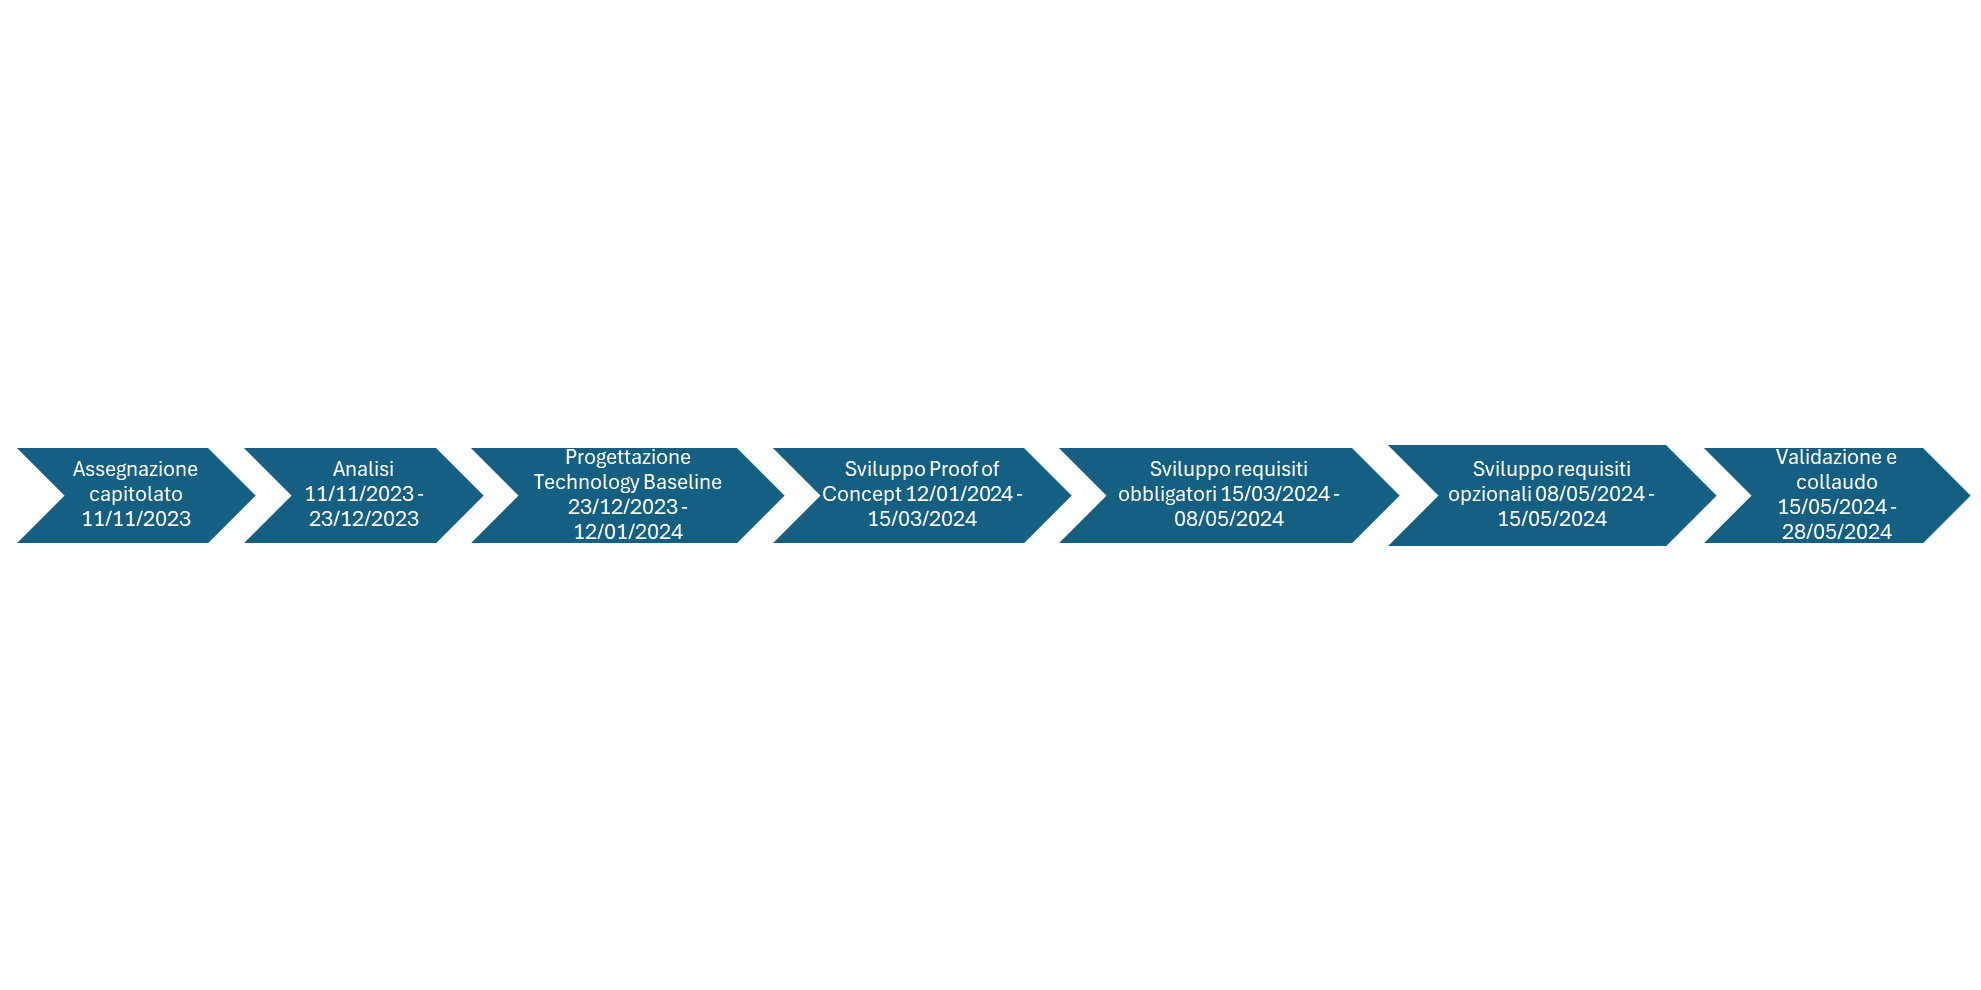
\includegraphics[width=18cm, height=5cm]{documenti/grafici/Sequenza temporale progetto.png}
\caption{Sequenza temporale del progetto}
\label{fig:STP}
\end{figure}

\subsubsection{Analisi}
\custombold{Periodo:} dal 11/11/2023 al 23/12/2023\\
Questo periodo inizia con l'assegnazione del capitolato d'appalto e termina all'inizio del periodo di Progettazione Technology Baseline\textsubscript{G}. Inizialmente vengono identificati gli strumenti per il lavoro collaborativo e quelli più adatti per la redazione della documentazione. Successivamente, si procede con un'analisi preliminare per individuare i requisiti necessari allo sviluppo del prodotto.\\
Durante questo periodo, data l'inesperienza del gruppo nelle tematiche trattate, si decide di dedicare tempo alla formazione. Inoltre, vengono redatti ulteriori documenti relativi alle strategie e alla qualità che il gruppo CyberSorceres si propone di rispettare.
\begin{itemize}
    \item \custombold{Formazione:} Tramite ore concordate con il proponente e tramite autoformazione tramite corsi online;
    \item \custombold{Norme del Way of Working:} Si procede con l'individuazione degli strumenti che saranno utilizzati per la stesura della documentazione e per la collaborazione. Le norme sono emanate dall'Amministratore e il rispetto di queste norme dovrà essere certificato dai verificatori. Viene quindi redatto il documento \textit{Norme Way of Working};
    \item \custombold{Piano di progetto:} Il Responsabile, basandosi sulle date concordate per le revisioni di avanzamento e sulle scadenze stabilite dal gruppo, redige il \textit{Piano di Progetto};
    \item \custombold{Analisi dei requisiti:} Utilizzando il capitolato d'appalto e attraverso incontri con il proponente, gli Analisti identificano i requisiti del sistema e redigono una prima versione dell'\textit{Analisi dei requisiti};
    \item \custombold{Piano di qualifica:} L'Amministratore redige i piani e le procedure di gestione per la qualità, mentre i verificatori illustrano l'esito e la completezza delle verifiche effettuate;
    \item \custombold{Glossario:} Viene redatto il \textit{Glossario}. Questo documento viene aggiornato in maniera continuativa.
\end{itemize}
\begin{figure}[H]
    \centering
    \includegraphics[width=\textwidth,height=\textheight,keepaspectratio]{documenti/grafici/diagramma-gantt-periodo-analisi.png}
    \caption{Diagramma di Gantt relativo al periodo di Analisi}
    \label{fig:GA}
\end{figure}

\subsubsection{Progettazione Technology Baseline}
\custombold{Periodo:} dal 23/12/2023 al 12/01/2024\\
Questo periodo inizia dopo l'Analisi e termina all'inizio della Codifica del Proof of Concept\textsubscript{G}. Al termine di questo periodo, è previsto un incontro con il proponente durante il quale verrà presentata la soluzione generale individuata e verranno annotati eventuali correzioni. Verranno inoltre apportati incrementi ai documenti prodotti nei periodi precedenti.\\
L'analisi del sistema effettuata in questo periodo serve come base tecnologica e progettuale per la codifica finale del Proof of Concept, che sarà realizzata nel periodo successivo.
\begin{itemize}
    \item \custombold{Technology Baseline:} In questa attività vengono studiate, analizzate e selezionate le tecnologie, i framework e le librerie da utilizzare nello sviluppo del prodotto;
    \item \custombold{Aggiornamento documentazione:} In questo periodo vengono apportate delle modifiche incrementali ai documenti precedentemente redatti.
\end{itemize}
\begin{figure}[H]
    \centering
    \includegraphics[width=\textwidth,height=\textheight,keepaspectratio]{documenti/grafici/diagramma-gantt-periodo-progettazione-technology-baseline.png}
    \caption{Diagramma di Gantt relativo al periodo di Progettazione Technology Baseline}
    \label{fig:GPTB}
\end{figure}

\subsubsection{Sviluppo Proof of Concept}
\custombold{Periodo:} dal 12/01/2024 al 7/03/2024\\
Questo periodo inizia dopo il periodo di Progettazione per la Technology Baseline e termina con la scadenza di consegna dei documenti per la revisione di Requirements and Technology Baseline (RTB\textsubscript{G}). L'attività principale di questo periodo è la realizzazione di un Proof of Concept\textsubscript{G}.
\begin{itemize}
    \item \custombold{Proof of Concept:} Il Proof of Concept è una dimostrazione eseguibile che servirà come base di partenza su cui effettuare incrementi nei periodi successivi;
    \item \custombold{Aggiornamento documentazione:} In questo periodo vengono apportate delle modifiche incrementali ai documenti precedentemente redatti.
\end{itemize}
\begin{figure}[H]
    \centering
    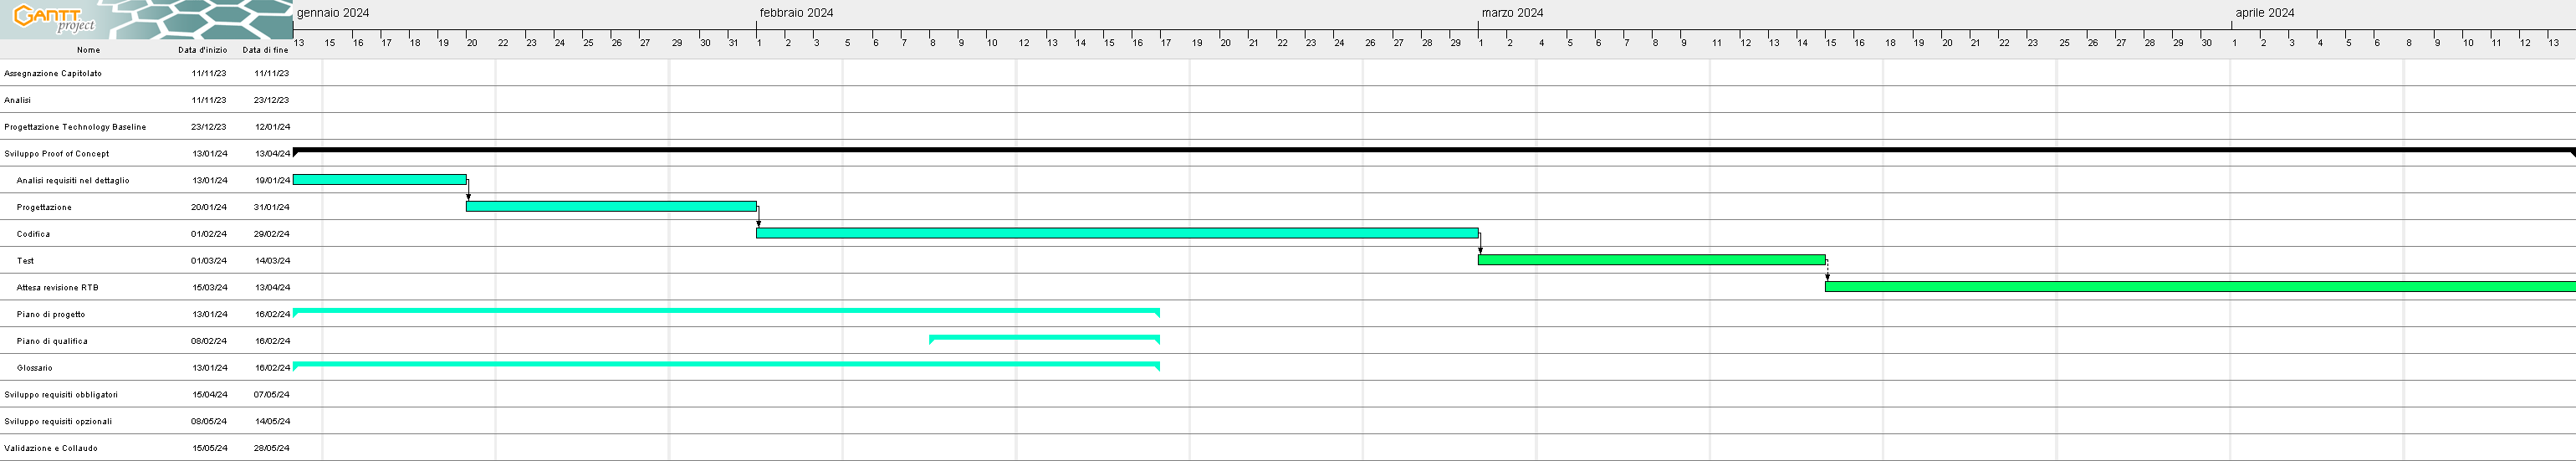
\includegraphics[width=\textwidth,height=\textheight,keepaspectratio]{documenti/grafici/diagramma-gantt-periodo-sviluppo-proof-of-concept.png}
    \caption{Diagramma di Gantt relativo al periodo di Sviluppo Proof of Concept}
    \label{fig:GSPOC}
\end{figure}

\subsubsection{Sviluppo requisiti obbligatori}
\custombold{Periodo:} dal 7/03/2024 al 30/03/2024\\
Questo periodo inizia dopo la revisione di Requirements and Technology Baseline (RTB\textsubscript{G}) e termina con l'inizio dello Sviluppo requisiti opzionali. Quindi, il Proof of Concept\textsubscript{G} precedentemente sviluppato sarà utilizzato come base per incrementare il prodotto. Una delle attività di questo periodo è la definizione della Product Baseline\textsubscript{G}.
\begin{itemize}
    \item \custombold{Product Baseline:} Questa attività illustra la baseline architetturale del prodotto attraverso i diagrammi delle classi, dimostrando la coerenza con quanto mostrato durante l'attività di Technology Baseline;
    \item \custombold{Test:} I Programmatori scrivono i test di unità e integrazione relativi ai componenti sviluppati in questo periodo;
    \item \custombold{Codifica:} Viene eseguito lo sviluppo del codice del prodotto da parte dei Programmatori relativamente ai componenti descritti dai requisiti obbligatori;
    \item \custombold{Manuale:} Comincia la redazione del documento \textit{Manuale Utente}. Questo documento fornisce indicazioni sull'utilizzo del sistema da parte degli utenti;
    \item \custombold{Aggiornamento documentazione:} In questo periodo vengono apportate delle modifiche incrementali ai documenti precedentemente redatti.
\end{itemize}
\begin{figure}[H]
    \centering
    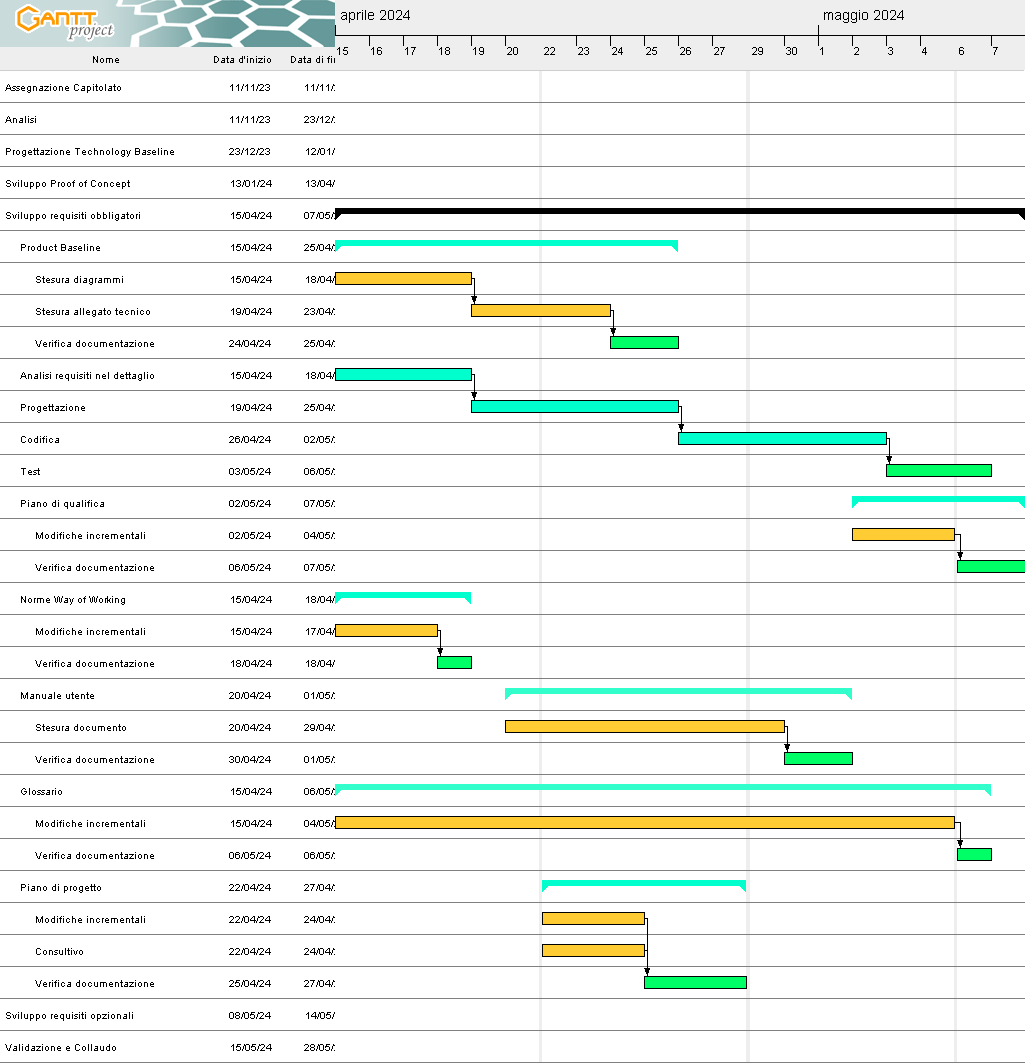
\includegraphics[width=\textwidth,height=\textheight,keepaspectratio]{documenti/grafici/diagramma-gantt-periodo-sviluppo-requisiti-obbligatori.png}
    \caption{Diagramma di Gantt relativo al periodo di Sviluppo Requisiti Obbligatori}
    \label{fig:GSRO}
\end{figure}

\subsubsection{Sviluppo requisiti opzionali}
\custombold{Periodo:} dal 1/04/2024 al 7/04/2024\\
Questo periodo inizia dopo lo Sviluppo requisiti obbligatori e termina con l'inizio dello periodo di Verifica e validazione. In preparazione alla revisione di Product Baseline (PB\textsubscript{G}), si procede con lo sviluppo dei requisiti opzionali.
\begin{itemize}
    \item \custombold{Test:} I Programmatori scrivono i test di unità e integrazione relativi ai componenti sviluppati in questo periodo;
    \item \custombold{Codifica:} Viene eseguito lo sviluppo del codice del prodotto da parte dei Programmatori relativamente ai componenti descritti dai requisiti opzionali;
    \item \custombold{Aggiornamento documentazione:} In questo periodo vengono apportate delle modifiche incrementali ai documenti precedentemente redatti.
\end{itemize}
\begin{figure}[H]
    \centering
    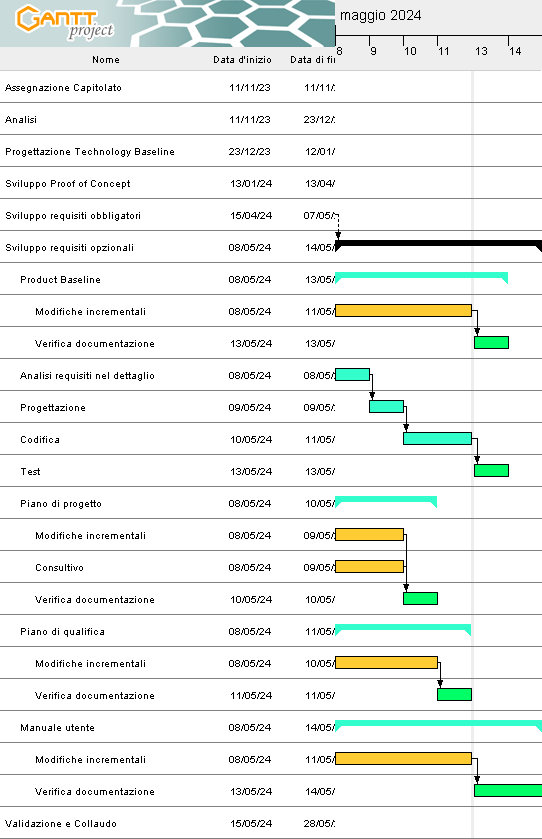
\includegraphics[width=\textwidth,height=\textheight,keepaspectratio]{documenti/grafici/diagramma-gantt-periodo-sviluppo-requisiti-opzionali.png}
    \caption{Diagramma di Gantt relativo al periodo di Sviluppo Requisiti Opzionali}
    \label{fig:GSROp}
\end{figure}

\subsubsection{Validazione e collaudo}
\custombold{Periodo:} dal 7/04/2024 al 28/04/2024\\
Questo periodo inizia dopo lo Sviluppo requisiti opzionali e termina con la scadenza di consegna dei documenti per la revisione di Customer Acceptance (CA\textsubscript{G}). Il sistema verrà collaudato e ci si assicurerà che il prodotto realizzato sia pienamente conforme alle aspettative.
\begin{itemize}
    \item \custombold{Test:} Oltre ai test di unità e integrazione, vengono eseguiti test di sistema;
    \item \custombold{Collaudo:} Il prodotto viene eseguito e testato in tutte le sue funzionalità, verificando che siano stati soddisfatti tutti i requisiti;
    \item \custombold{Validazione:} Viene verificato che il prodotto sia conforme alle specifiche e soddisfi le richieste del cliente;
    \item \custombold{Aggiornamento documentazione:} In questo periodo vengono apportate delle modifiche incrementali ai documenti precedentemente redatti.
\end{itemize}
\begin{figure}[H]
    \centering
    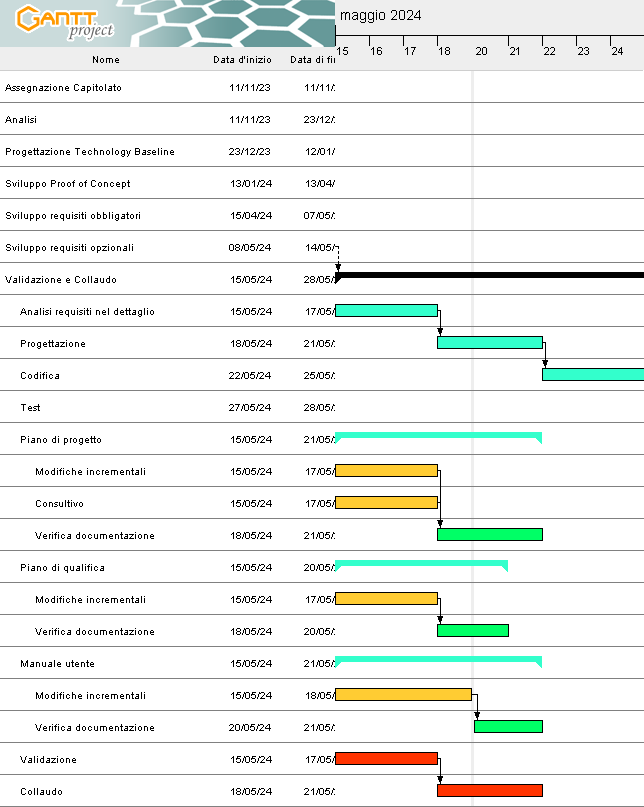
\includegraphics[width=\textwidth,height=\textheight,keepaspectratio]{documenti/grafici/diagramma-gantt-periodo-valida-e-collaudo.png}
    \caption{Diagramma di Gantt relativo al periodo di Validazione e Collaudo}
    \label{fig:GVC}
\end{figure}
\newpage
\section{Preventivo}
Ogni membro del gruppo può assumere più di un ruolo, sia contemporaneamente che in fasi diverse del progetto, a condizione che non vi sia un conflitto di interessi tra i ruoli assunti. La divisione del lavoro che sarà illustrata di seguito assicurerà una distribuzione equa del carico di lavoro individuale e dei vari ruoli.\\
\\
Nelle tabelle saranno impiegate abbreviazioni per indicare i nomi dei ruoli, secondo quanto specificato nella seguente tabella:
\begin{center}
    \begin{tabular}{c|c}
    \rowcolor{Blue}
    \custombold{Ruolo} & \custombold{Abbreviazione}\\
    \rowcolor{LighterBlue}
    \custombold{Responsabile} & Re\\
    \rowcolor{LightBlue}
    \custombold{Amministratore} & Am\\
    \rowcolor{LighterBlue}
    \custombold{Analista} & An\\
    \rowcolor{LightBlue}
    \custombold{Progettista} & Pt\\
    \rowcolor{LighterBlue}
    \custombold{Programmatore} & Pr\\
    \rowcolor{LightBlue}
    \custombold{Verificatore} & Ve\\
    \end{tabular}
    \captionof{table}{Abbreviazioni dei ruoli}
\label{tab:ruoli}
\end{center}
\subsection{Riepilogo economico e delle ore - Periodo Analisi}
Durante il periodo di Analisi, ciascun membro assumerà i ruoli secondo la seguente distribuzione:\\
\\
\begin{center}
\begin{tabular}{c|c|c|c|c|c|c|c}
\rowcolor{Blue}
\custombold{Nominativo} & \custombold{Re} & \custombold{Am} & \custombold{An} & \custombold{Pt} & \custombold{Pr} & \custombold{Ve} & \custombold{Ore Totali}\\
\hline
\rowcolor{LighterBlue}
Sabrina Caniato & 9 & 0 & 14 & 0 & 0 & 5 & 28\\
\rowcolor{LightBlue}
Giulia Dentone & 0 & 12 & 13 & 0 & 0 & 5 & 30\\
\rowcolor{LighterBlue}
Nicola Lazzarin & 0 & 12 & 14 & 0 & 0 & 5 & 31\\
\rowcolor{LightBlue}
Giovanni Moretti & 12 & 0 & 15 & 0 & 0 & 5 & 32\\
\rowcolor{LighterBlue}
Andrea Rezzi & 8 & 0 & 14 & 0 & 0 & 5 & 27\\
\rowcolor{LightBlue}
Samuele Vignotto & 0 & 12 & 11 & 0 & 0 & 5 & 28\\
\rowcolor{LighterBlue}
\custombold{Ore totali} & 29 & 36 & 81 & 0 & 0 & 30 & 176\\
\end{tabular}
\captionof{table}{Preventivo ore per l'analisi}
\label{tab:preventivoAnalisi}
\end{center}


\begin{figure}[h]
    \centering
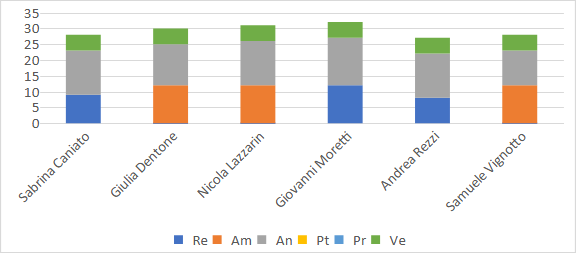
\includegraphics[width=17cm, height=10cm]{documenti/grafici/Divisione_ore_lavorative_Analisi.png}    
    \caption{Grafico divisione ore lavorative periodo di Analisi}
    \label{fig:preventivoAnalisi}
\end{figure}

\newpage

In questo periodo i costi da affrontare sono:
\begin{center}
    \begin{tabular}{c|c|c}
    \rowcolor{Blue}
    \custombold{Ruolo} & \custombold{Ore} & \custombold{Costo \euro}\\
    \rowcolor{LighterBlue}
    Responsabile & 29 & 870\\
    \rowcolor{LightBlue}
    Amministratore & 36 & 720\\
    \rowcolor{LighterBlue}
    Analista & 81 & 2025\\
    \rowcolor{LightBlue}
    Progettista & 0 & 0\\
    \rowcolor{LighterBlue}
    Programmatore & 0 & 0\\
    \rowcolor{LightBlue}
    Verificatore & 30 & 450\\
    \rowcolor{LighterBlue}
    \custombold{Totale} & \custombold{176} & \custombold{4065}\\
    \end{tabular}
    \captionof{table}{Costi nel periodo di Analisi}
    \label{tab:costiAnalisi}
\end{center}

\begin{figure}[h]
    \centering
    \includegraphics[width=17cm, height=10cm]{documenti/grafici/Torta_percentuale_costi_Analisi.jpg}
    \caption{grafico della divisione percentuale dei costi sostenuti nel periodo di Analisi}
    \label{fig:enter-label}
\end{figure}


\newpage

\subsection{Riepilogo economico e delle ore parziale - Periodo Progettazione Technology Baseline\textsubscript{G}}
Durante il periodo di Progettazione Technology Baseline\textsubscript{G}, ciascun membro assumerà i ruoli secondo la seguente distribuzione:\\
\\
\begin{center}
\begin{tabular}{c|c|c|c|c|c|c|c}
\rowcolor{Blue}
\custombold{Nominativo} & \custombold{Re} & \custombold{Am} & \custombold{An} & \custombold{Pt} & \custombold{Pr} & \custombold{Ve} & \custombold{Ore Totali}\\
\hline
\rowcolor{LighterBlue}
Sabrina Caniato & 0 & 0 & 4 & 11 & 0 & 2 & 17\\
\rowcolor{LightBlue}
Giulia Dentone & 0 & 0 & 3 & 5 & 0 & 2 & 10\\
\rowcolor{LighterBlue}
Nicola Lazzarin & 0 & 0 & 4 & 6 & 0 & 2 & 12\\
\rowcolor{LightBlue}
Giovanni Moretti & 0 & 3 & 1 & 4 & 0 & 2 & 10\\
\rowcolor{LighterBlue}
Andrea Rezzi & 0 & 8 & 4 & 3 & 0 & 2 & 17\\
\rowcolor{LightBlue}
Samuele Vignotto & 12 & 0 & 0 & 2 & 0 & 2 & 16\\
\rowcolor{LighterBlue}
\custombold{Ore totali} & 12 & 11 & 16 & 31 & 0 & 12 & 82\\
\end{tabular}
\captionof{table}{Preventivo ore Progettazione Technology Baseline}
\label{tab:PTB}
\end{center}

\begin{figure}[h]
    \centering
    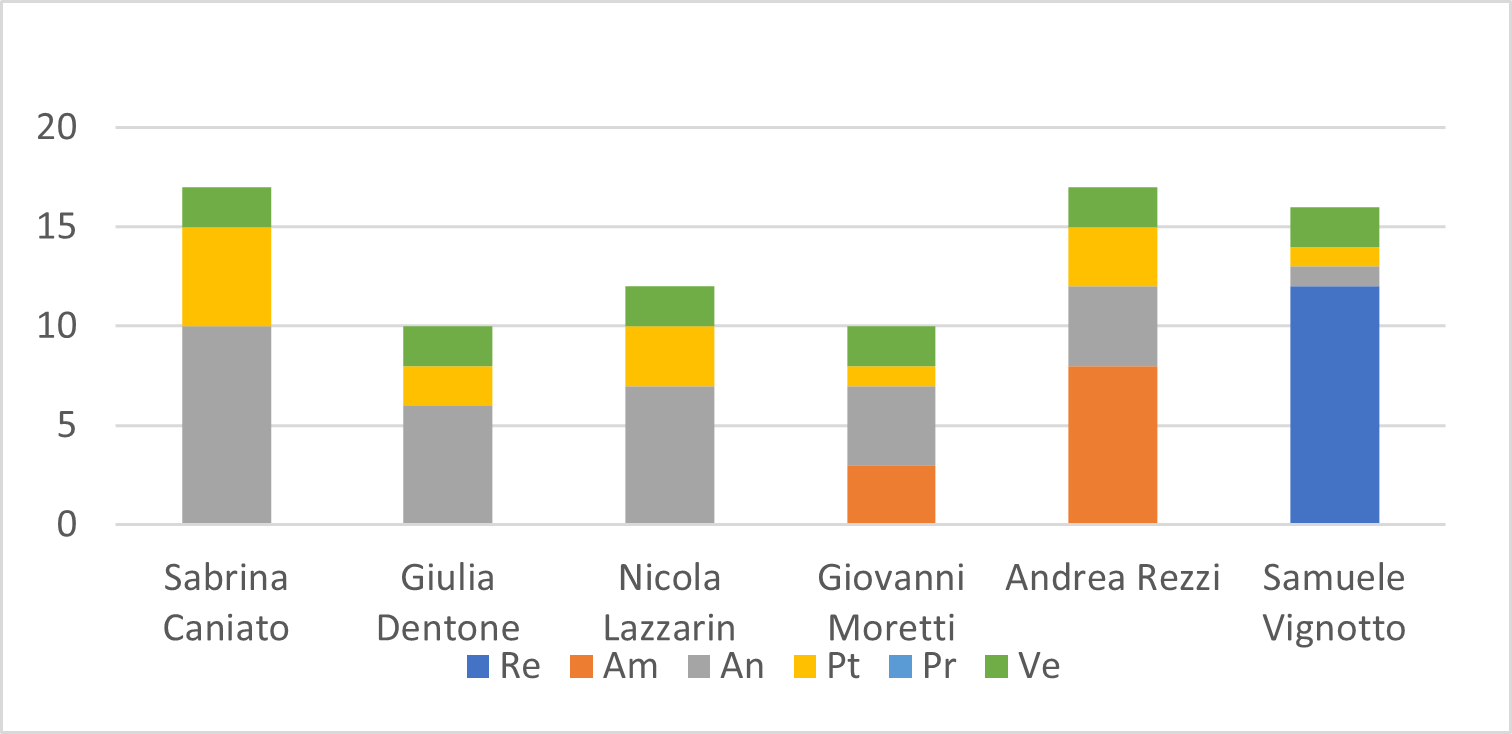
\includegraphics[width=17cm, height=10cm]{documenti/grafici/Divisione_ore_lavorative_Progettazione_Technology_Baseline.png}
    \caption{Grafico divisione ore lavorative periodo di Progettazione Techonology Baseline}
    \label{fig:PTB}
\end{figure}

\newpage
In questo periodo i costi da affrontare sono:
\begin{center}
    \begin{tabular}{c|c|c}
    \rowcolor{Blue}
    \custombold{Ruolo} & \custombold{Ore} & \custombold{Costo \euro}\\
    \rowcolor{LighterBlue}
    Responsabile & 12 & 360\\
    \rowcolor{LightBlue}
    Amministratore & 11 & 220\\
    \rowcolor{LighterBlue}
    Analista & 16 & 400\\
    \rowcolor{LightBlue}
    Progettista & 31 & 775\\
    \rowcolor{LighterBlue}
    Programmatore & 0 & 0\\
    \rowcolor{LightBlue}
    Verificatore & 12 & 180\\
    \rowcolor{LighterBlue}
    \custombold{Totale} & \custombold{82} & \custombold{1935}\\
    \end{tabular}
    \captionof{table}{Preventivo costi Progettazione Technology Baseline}
\label{tab:costiPTB}
\end{center}

\begin{figure}[h]
    \centering
    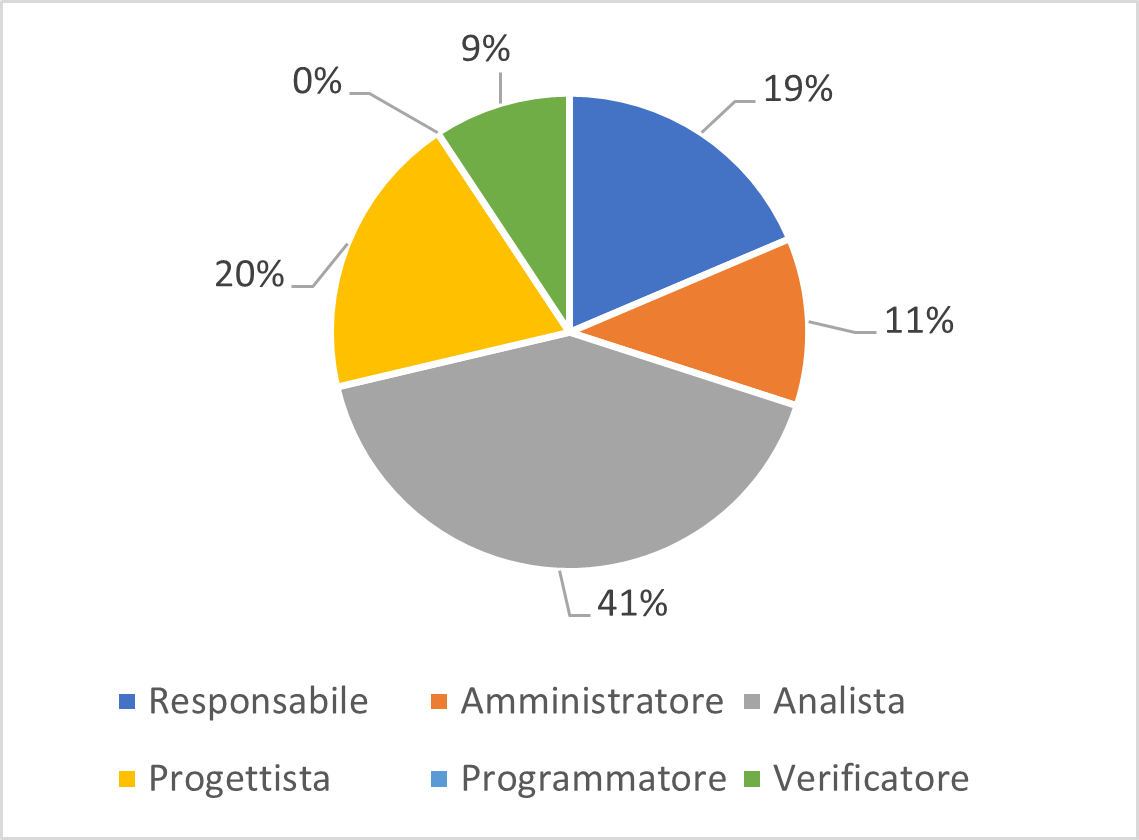
\includegraphics[width=17cm, height=10cm]{documenti/grafici/Torta_percentuale_costi_Progettazione_Technology_Baseline.jpg}
 \caption{grafico della divisione percentuale dei costi sostenuti nel periodo di Progettazione Technology Baseline}
    \label{fig:costiPTB}
\end{figure}
   
\newpage

\subsection{Riepilogo economico e delle ore parziale - Periodo Sviluppo Proof of Concept\textsubscript{G}}
Durante il periodo di Sviluppo Proof of Concept\textsubscript{G}, ciascun membro assumerà i ruoli secondo la seguente distribuzione:\\
\\
\begin{center}
\begin{tabular}{c|c|c|c|c|c|c|c}
\rowcolor{Blue}
\custombold{Nominativo} & \custombold{Re} & \custombold{Am} & \custombold{An} & \custombold{Pt} & \custombold{Pr} & \custombold{Ve} & \custombold{Ore Totali}\\
\hline
\rowcolor{LighterBlue}
Sabrina Caniato & 0 & 0 & 0 & 4 & 6 & 2 & 12\\
\rowcolor{LightBlue}
Giulia Dentone & 12 & 0 & 0 & 2 & 5 & 2 & 21\\
\rowcolor{LighterBlue}
Nicola Lazzarin & 0 & 0 & 0 & 4 & 9 & 2 & 15\\
\rowcolor{LightBlue}
Giovanni Moretti & 0 & 5 & 0 & 3 & 7 & 2 & 17\\
\rowcolor{LighterBlue}
Andrea Rezzi & 0 & 0 & 0 & 6 & 8 & 2 & 16\\
\rowcolor{LightBlue}
Samuele Vignotto & 0 & 0 & 7 & 4 & 5 & 2 & 18\\
\rowcolor{LighterBlue}
\custombold{Ore totali} & 12 & 5 & 7 & 23 & 40 & 12 & 99\\
\end{tabular}
    \captionof{table}{Preventivo ore Proof of Concept}
\label{tab:POC}
\end{center}

\begin{figure}[h]
    \centering
    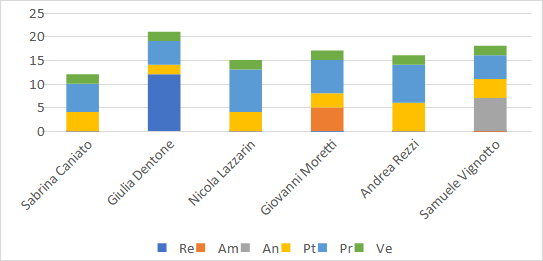
\includegraphics[width=17cm, height=10cm]{documenti/grafici/Divisione_ore_lavorative_Sviluppo_Proof_of_Concept.png}    \caption{Grafico divisione ore lavorative periodo di Sviluppo Proof of Concept}
    \label{fig:POC}
\end{figure}


\newpage
In questo periodo i costi da affrontare sono:
\begin{center}
    \begin{tabular}{c|c|c}
    \rowcolor{Blue}
    \custombold{Ruolo} & \custombold{Ore} & \custombold{Costo \euro}\\
    \rowcolor{LighterBlue}
    Responsabile & 12 & 360\\
    \rowcolor{LightBlue}
    Amministratore & 5 & 100\\
    \rowcolor{LighterBlue}
    Analista & 7 & 175\\
    \rowcolor{LightBlue}
    Progettista & 23 & 575\\
    \rowcolor{LighterBlue}
    Programmatore & 40 & 600\\
    \rowcolor{LightBlue}
    Verificatore & 12 & 180\\
    \rowcolor{LighterBlue}
    \custombold{Totale} & \custombold{99} & \custombold{1990}\\
    \end{tabular}
        \captionof{table}{Preventivo costi Proof of Concept}
\label{tab:costiPOC}
\end{center}
\begin{figure}[h]
    \centering
\includegraphics[width=17cm, height=10cm]{documenti/grafici/Torta_percentuali_costi_Sviluppo_Proof_of_Concept.jpg}    \caption{Grafico della divisione percentuale dei costi sostenuti nel periodo di Sviluppo Proof of Concept}
    \label{fig:enter-label}
\end{figure}

\newpage

\subsection{Riepilogo economico e delle ore parziale - Periodo Sviluppo Requisiti Obbligatori}
Durante il periodo di Sviluppo Requisiti Obbligatori, ciascun membro assumerà i ruoli secondo la seguente distribuzione:\\
\\
\begin{center}
\begin{tabular}{c|c|c|c|c|c|c|c}
\rowcolor{Blue}
\custombold{Nominativo} & \custombold{Re} & \custombold{Am} & \custombold{An} & \custombold{Pt} & \custombold{Pr} & \custombold{Ve} & \custombold{Ore Totali}\\
\hline
\rowcolor{LighterBlue}
Sabrina Caniato & 0 & 7 & 0 & 2 & 6 & 2 & 17\\
\rowcolor{LightBlue}
Giulia Dentone & 0 & 0 & 0 & 4 & 6 & 2 & 12\\
\rowcolor{LighterBlue}
Nicola Lazzarin & 7 & 0 & 0 & 4 & 0 & 2 & 13\\
\rowcolor{LightBlue}
Giovanni Moretti & 0 & 0 & 2 & 3 & 6 & 2 & 13\\
\rowcolor{LighterBlue}
Andrea Rezzi & 0 & 0 & 0 & 3 & 7 & 2 & 12\\
\rowcolor{LightBlue}
Samuele Vignotto & 0 & 0 & 0 & 4 & 6 & 2 & 12\\
\rowcolor{LighterBlue}
\custombold{Ore totali} & 7 & 7 & 2 & 20 & 31 & 12 & 79\\
\end{tabular}
        \captionof{table}{Preventivo ore Periodo Sviluppo Requisiti Obligatori}
\label{tab:PSRO}
\end{center}

\begin{figure}[h]
    \centering
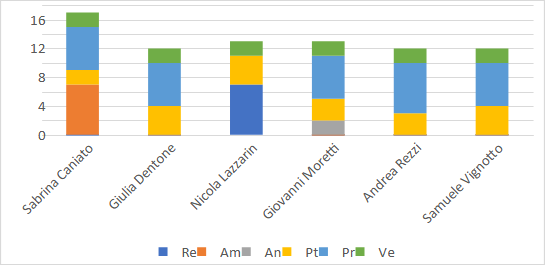
\includegraphics[width=17cm, height=10cm]{documenti/grafici/Divisione_ore_lavorative_Sviluppo_Requisiti_Obbligatori.png}    \caption{Grafico divisione ore lavorative periodo di Sviluppo Requisiti Obbligatori}
    \label{fig:PSRO}
\end{figure}

\newpage
In questo periodo i costi da affrontare sono:
\begin{center}
    \begin{tabular}{c|c|c}
    \rowcolor{Blue}
    \custombold{Ruolo} & \custombold{Ore} & \custombold{Costo \euro}\\
    \rowcolor{LighterBlue}
    Responsabile & 7 & 210\\
    \rowcolor{LightBlue}
    Amministratore & 7 & 140\\
    \rowcolor{LighterBlue}
    Analista & 2 & 50\\
    \rowcolor{LightBlue}
    Progettista & 20 & 500\\
    \rowcolor{LighterBlue}
    Programmatore & 31 & 465\\
    \rowcolor{LightBlue}
    Verificatore & 12 & 180\\
    \rowcolor{LighterBlue}
    \custombold{Totale} & \custombold{79} & \custombold{1545}\\
    \end{tabular}
    \captionof{table}{Preventivo costi Periodo Sviluppo Requisiti Obligatori}
\label{tab:costiPSRO}
\end{center}

\begin{figure}[h]
    \centering
    \includegraphics[width=17cm, height=10cm]{documenti/grafici/Torta_percentuale_costi_Sviluppo_Requisiti_Obbligatori.jpg}    
    \caption{Grafico della divisione percentuale dei costi sostenuti nel periodo di Sviluppo Requisiti Obbligatori}
    \label{fig:costiPSRO}
\end{figure}

\newpage

\subsection{Riepilogo economico e delle ore parziale - Periodo Sviluppo Requisiti Opzionali}
Durante il periodo di Sviluppo Requisiti Opzionali, ciascun membro assumerà i ruoli secondo la seguente distribuzione:\\
\\
\begin{center}
\begin{tabular}{c|c|c|c|c|c|c|c}
\rowcolor{Blue}
\custombold{Nominativo} & \custombold{Re} & \custombold{Am} & \custombold{An} & \custombold{Pt} & \custombold{Pr} & \custombold{Ve} & \custombold{Ore Totali}\\
\hline
\rowcolor{LighterBlue}
Sabrina Caniato & 0 & 3 & 0 & 0 & 4 & 2 & 9\\
\rowcolor{LightBlue}
Giulia Dentone & 0 & 0 & 2 & 0 & 5 & 2 & 9\\
\rowcolor{LighterBlue}
Nicola Lazzarin & 5 & 0 & 0 & 0 & 5 & 2 & 12\\
\rowcolor{LightBlue}
Giovanni Moretti & 0 & 0 & 0 & 4 & 5 & 2 & 11\\
\rowcolor{LighterBlue}
Andrea Rezzi & 0 & 2 & 0 & 3 & 4 & 2 & 11\\
\rowcolor{LightBlue}
Samuele Vignotto & 0 & 0 & 0 & 4 & 4 & 2 & 10\\
\rowcolor{LighterBlue}
\custombold{Ore totali} & 5 & 5 & 2 & 11 & 27 & 12 & 62\\
\end{tabular}
   \captionof{table}{Preventivo ore Periodo Sviluppo Requisiti Opzionali}
\label{tab:PSROp}
\end{center}
\begin{figure}[h]
    \centering
    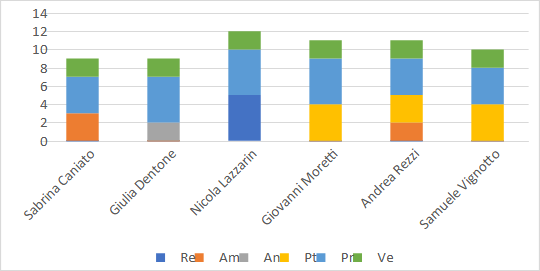
\includegraphics[width=17cm, height=10cm]{documenti/grafici/Divisione_ore_lavorative_Sviluppo_Requisiti_Opzionali.png}\caption{ Grafico divisione ore lavorative periodo di Sviluppo Requisiti Opzionali}
    \label{fig:PSROp}
\end{figure}

\newpage
In questo periodo i costi da affrontare sono:
\begin{center}
    \begin{tabular}{c|c|c}
    \rowcolor{Blue}
    \custombold{Ruolo} & \custombold{Ore} & \custombold{Costo \euro}\\
    \rowcolor{LighterBlue}
    Responsabile & 5 & 150\\
    \rowcolor{LightBlue}
    Amministratore & 5 & 100\\
    \rowcolor{LighterBlue}
    Analista & 2 & 50\\
    \rowcolor{LightBlue}
    Progettista & 11 & 275\\
    \rowcolor{LighterBlue}
    Programmatore & 27 & 405\\
    \rowcolor{LightBlue}
    Verificatore & 12 & 180\\
    \rowcolor{LighterBlue}
    \custombold{Totale} & \custombold{62} & \custombold{1160}\\
    \end{tabular}
       \captionof{table}{Preventivo costi Periodo Sviluppo Requisiti Opzionali}
\label{tab:costiPSROp}
\end{center}
\begin{figure}[h]
    \centering
    \includegraphics[width=17cm, height=10cm]{documenti/grafici/Torta_percentuale_costi_Sviluppo_Requisiti_Opzionali.jpg} \caption{Grafico della divisione percentuale dei costi sostenuti nel periodo di Sviluppo Requisiti Opzionali}
    \label{fig:costiPSROp}
\end{figure}

\newpage

\subsection{Riepilogo economico e delle ore parziale - Periodo Validazione E Collaudo}
Durante il periodo di Validazione e Collaudo, ciascun membro assumerà i ruoli secondo la seguente distribuzione:\\
\\
\begin{center}
\begin{tabular}{c|c|c|c|c|c|c|c}
\rowcolor{Blue}
\custombold{Nominativo} & \custombold{Re} & \custombold{Am} & \custombold{An} & \custombold{Pt} & \custombold{Pr} & \custombold{Ve} & \custombold{Ore Totali}\\
\hline
\rowcolor{LighterBlue}
Sabrina Caniato & 3 & 2 & 0 & 0 & 5 & 2 & 12\\
\rowcolor{LightBlue}
Giulia Dentone & 0 & 0 & 0 & 6 & 5 & 2 & 13\\
\rowcolor{LighterBlue}
Nicola Lazzarin & 0 & 0 & 0 & 3 & 7 & 2 & 12\\
\rowcolor{LightBlue}
Giovanni Moretti & 0 & 4 & 0 & 3 & 3 & 2 & 12\\
\rowcolor{LighterBlue}
Andrea Rezzi & 4 & 2 & 0 & 2 & 2 & 2 & 12\\
\rowcolor{LightBlue}
Samuele Vignotto & 0 & 0 & 0 & 3 & 6 & 2 & 11\\
\rowcolor{LighterBlue}
\custombold{Ore totali} & 7 & 8 & 0 & 17 & 28 & 12 & 72\\
\end{tabular}
       \captionof{table}{Preventivo ore Periodo Validazione e Collaudo}
\label{tab:PVC}
\end{center}

\begin{figure}[h]
    \centering
    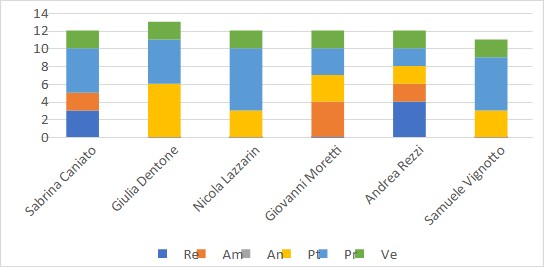
\includegraphics[width=17cm, height=10cm]{documenti/grafici/Divisione_ore_lavorative_Validazione_e_Collaudo.png}    \caption{Grafico divisione ore lavorative periodo di Validazione e Collaudo}
    \label{fig:PVC}
\end{figure}

\newpage
In questo periodo i costi da affrontare sono:
\begin{center}
    \begin{tabular}{c|c|c}
    \rowcolor{Blue}
    \custombold{Ruolo} & \custombold{Ore} & \custombold{Costo \euro}\\
    \rowcolor{LighterBlue}
    Responsabile & 7 & 210\\
    \rowcolor{LightBlue}
    Amministratore & 8 & 160\\
    \rowcolor{LighterBlue}
    Analista & 0 & 0\\
    \rowcolor{LightBlue}
    Progettista & 17 & 425\\
    \rowcolor{LighterBlue}
    Programmatore & 28 & 420\\
    \rowcolor{LightBlue}
    Verificatore & 12 & 180\\
    \rowcolor{LighterBlue}
    \custombold{Totale} & \custombold{72} & \custombold{1395}\\
    \end{tabular}
    \captionof{table}{Preventivo costi Periodo Validazione e Collaudo}
\label{tab:costiPVC}
\end{center}

\begin{figure}[h]
    \centering
    \includegraphics[width=17cm, height=10cm]{documenti/grafici/Torta_percentuale_costi_Validazione_e_Collaudo.jpg}    \caption{Grafico della divisione percentuale dei costi sostenuti nel periodo di Validazione e Collaudo}
    \label{fig:costiPVC}
\end{figure}

\newpage

\subsection{Riepilogo economico e delle ore totale}
I costi e le ore totali vengono riassunti nella seguente tabella:
\begin{center}
    \begin{tabular}{c|c|c|c|c}
    \rowcolor{Blue}
    \custombold{Ruolo} & \custombold{Costo orario} & \custombold{Ore per ruolo} & \custombold{Ore per membro} & \custombold{Costo totale}\\
    \rowcolor{LighterBlue}
    Responsabile & 30 & 72 & 12 & 2160\\
    \rowcolor{LightBlue}
    Amministratore & 20 & 72 & 12 & 1440\\
    \rowcolor{LighterBlue}
    Analista & 25 & 108 & 18 & 2700\\
    \rowcolor{LightBlue}
    Progettista & 25 & 102 & 17 & 2550\\
    \rowcolor{LighterBlue}
    Programmatore & 15 & 126 & 21 & 1890\\
    \rowcolor{LightBlue}
    Verificatore & 15 & 90 & 15 & 1350\\
    \rowcolor{LighterBlue}
    \custombold{Totale} & - & 570 & 95 & 12090\\
    \end{tabular}
    \captionof{table}{Preventivo ore totali}
\label{tab:ore}
\end{center}
\newpage

\section{Consuntivo}
Questa sezione presenta le spese effettivamente sostenute dal team Cyber Sorceres. Vengono dettagliate le ore e i costi associati a ciascun ruolo per l'esecuzione delle attività pianificate. Inoltre, è fornito un bilancio finanziario che rappresenta la differenza tra il consuntivo di periodo e il preventivo. Tale bilancio può assumere le seguenti condizioni:
\begin{itemize}
    \item \custombold{Positivo}: se la spesa effettiva è inferiore a quanto preventivato;
    \item \custombold{Pareggio}: se la spesa effettiva è uguale a quanto preventivato;
    \item \custombold{Negativo}: se la spesa effettiva è maggiore a quanto preventivato.
\end{itemize}
Il bilancio è indicato tra parentesi accanto ai valori rilevati dal consuntivo di periodo. Se il valore tra parentesi è assente, ciò indica che l'aspettativa del preventivo è stata rispettata.

\subsection{Periodo di Analisi}
\subsubsection{Variazione della pianificazione}
\begin{center}
\begin{tabular}{c|c|c|c|c|c|c|c}
\rowcolor{Blue}
\custombold{Nominativo} & \custombold{Re} & \custombold{Am} & \custombold{An} & \custombold{Pt} & \custombold{Pr} & \custombold{Ve} & \custombold{Ore Totali}\\
\hline
\rowcolor{LighterBlue}
Sabrina Caniato & 9 (+2) & 0 & 14 & 0 & 0 & 5 & 28\\
\rowcolor{LightBlue}
Giulia Dentone & 0 & 12 & 13(-3) & 0 & 0 & 5 & 30\\
\rowcolor{LighterBlue}
Nicola Lazzarin & 0 & 12(-2) & 14 & 0 & 0 & 5 & 31\\
\rowcolor{LightBlue}
Giovanni Moretti & 12 & 0 & 15(+2) & 0 & 0 & 5 & 32\\
\rowcolor{LighterBlue}
Andrea Rezzi & 8 & 0 & 14(-2) & 0 & 0 & 5 & 27\\
\rowcolor{LightBlue}
Samuele Vignotto & 0 & 12(+1) & 11 & 0 & 0 & 5 & 28\\
\rowcolor{LighterBlue}
\custombold{Ore totali} & 29(+2) & 36(-1) & 81(-3) & 0 & 0 & 30 & 176(-2)\\
\end{tabular}
\captionof{table}{Variazione pianificazione nell'analisi}
\label{tab:varPian}
\end{center}
\subsubsection{Variazione dei costi}
\begin{center}
    \begin{tabular}{c|c|c}
    \rowcolor{Blue}
    \custombold{Ruolo} & \custombold{Ore} & \custombold{Costo \euro}\\
    \rowcolor{LighterBlue}
    Responsabile & 29(+2) & 870(+50)\\
    \rowcolor{LightBlue}
    Amministratore & 36(-1) & 720(-20)\\
    \rowcolor{LighterBlue}
    Analista & 81(-3) & 2025(-75)\\
    \rowcolor{LightBlue}
    Progettista & 0 & 0\\
    \rowcolor{LighterBlue}
    Programmatore & 0 & 0\\
    \rowcolor{LightBlue}
    Verificatore & 30 & 450\\
    \rowcolor{LighterBlue}
    \custombold{Totale} & \custombold{176(-2)} & \custombold{4065(-35)}\\
    \end{tabular}
    \captionof{table}{Variazione costi nell'analisi}
\label{tab:varCosti}
\end{center}
\subsubsection{Ragione degli scostamenti}
\begin{itemize}
    \item \custombold{Responsabile}: inesperienza nel ricoprire tale ruolo;
    \item \custombold{Amministratore}: esperienze pregresse di un membro del gruppo;
    \item \custombold{Analista}: il proponente ha fornito al gruppo molto supporto nella stesura dell'\textit{Analisi dei Requisiti}.
\end{itemize}
\subsubsection{Considerazioni rispetto al preventivo}
Il bilancio evidenzia un risultato positivo rispetto al preventivo per questo periodo. Tuttavia, non si ritiene necessaria alcuna ripianificazione per il prossimo periodo, poiché l'importo risparmiato non è considerato significativo. Inoltre, poiché sono stati raggiunti tutti gli obiettivi precedentemente pianificati, non si è verificato alcun rallentamento nell'avanzamento delle attività.

\subsection{Periodo di Progettazione Technology Baseline\textsubscript{G}}
\subsubsection{Variazione della pianificazione}
\begin{center}
\begin{tabular}{c|c|c|c|c|c|c|c}
\rowcolor{Blue}
\custombold{Nominativo} & \custombold{Re} & \custombold{Am} & \custombold{An} & \custombold{Pt} & \custombold{Pr} & \custombold{Ve} & \custombold{Ore Totali}\\
\hline
\rowcolor{LighterBlue}
Sabrina Caniato & 0 & 0 & 4 & 11 & 0 & 2 & 17\\
\rowcolor{LightBlue}
Giulia Dentone & 0 & 0 & 3 & 5(+3) & 0 & 2 & 10\\
\rowcolor{LighterBlue}
Nicola Lazzarin & 0 & 0 & 4 & 6 & 0 & 2 & 12\\
\rowcolor{LightBlue}
Giovanni Moretti & 0 & 3 & 1 & 4(+1) & 0 & 2 & 10\\
\rowcolor{LighterBlue}
Andrea Rezzi & 0 & 8 & 4 & 3(+2) & 0 & 2 & 17\\
\rowcolor{LightBlue}
Samuele Vignotto & 12 & 0 & 0 & 2(+4) & 0 & 2 & 16\\
\rowcolor{LighterBlue}
\custombold{Ore totali} & 12 & 11 & 16 & 31(+10) & 0 & 12 & 82(+10)\\
\end{tabular}
\captionof{table}{Variazione pianificazione del periodo di progettazione Technology Beseline}
\label{tab:varPTB}
\end{center}
\subsubsection{Variazione dei costi}
\begin{center}
    \begin{tabular}{c|c|c}
    \rowcolor{Blue}
    \custombold{Ruolo} & \custombold{Ore} & \custombold{Costo \euro}\\
    \rowcolor{LighterBlue}
    Responsabile & 12 & 360\\
    \rowcolor{LightBlue}
    Amministratore & 11 & 220\\
    \rowcolor{LighterBlue}
    Analista & 16 & 400\\
    \rowcolor{LightBlue}
    Progettista & 31(+10) & 775(+250)\\
    \rowcolor{LighterBlue}
    Programmatore & 0 & 0\\
    \rowcolor{LightBlue}
    Verificatore & 12 & 180\\
    \rowcolor{LighterBlue}
    \custombold{Totale} & \custombold{82(+10)} & \custombold{1935+250}\\
    \end{tabular}
    \captionof{table}{Variazione costi del periodo di progettazione Technology Beseline}
\label{tab:varPTB}
\end{center}
\subsubsection{Ragione degli scostamenti}
\begin{itemize}
    \item \custombold{Progettista}: nessuna esperienza con gli strumenti forniti dal proponente.
\end{itemize}
\subsubsection{Considerazioni rispetto al preventivo}
Il bilancio risulta negativo, ma il gruppo conta di recuperare nelle prossime fasi del progetto poiché ha maggiore esperienza.

\subsection{Periodo di Sviluppo Proof of Concept - a finire}
\subsubsection{Prospetto orario}
\begin{center}
\begin{tabular}{c|c|c|c|c|c|c|c}
\rowcolor{Blue}
\custombold{Nominativo} & \custombold{Re} & \custombold{Am} & \custombold{An} & \custombold{Pt} & \custombold{Pr} & \custombold{Ve} & \custombold{Ore Totali}\\
\hline
\rowcolor{LighterBlue}
Sabrina Caniato & 0 & 0 & 0 & 4 & 6 & 2 & 12\\
\rowcolor{LightBlue}
Giulia Dentone & 12 & 0 & 0 & 2 & 5 & 2 & 21\\
\rowcolor{LighterBlue}
Nicola Lazzarin & 0 & 0 & 0 & 4 & 9(-2) & 2 & 15\\
\rowcolor{LightBlue}
Giovanni Moretti & 0 & 5 & 0 & 3 & 7 & 2 & 17\\
\rowcolor{LighterBlue}
Andrea Rezzi & 0 & 0 & 0 & 6(-2) & 8(-2) & 2 & 16\\
\rowcolor{LightBlue}
Samuele Vignotto & 0 & 0 & 7 & 4 & 5(-1) & 2 & 18\\
\rowcolor{LighterBlue}
\custombold{Ore totali} & 12 & 5 & 7 & 23(-2) & 40(-4) & 12 & 99(-6)\\
\end{tabular}
\captionof{table}{Variazione pianificazione del periodo di sviluppo del proof of concept}
\label{tab:varPOC}
\end{center}
\subsubsection{Prospetto economico}
\begin{center}
    \begin{tabular}{c|c|c}
    \rowcolor{Blue}
    \custombold{Ruolo} & \custombold{Ore} & \custombold{Costo \euro}\\
    \rowcolor{LighterBlue}
    Responsabile & 12 & 360\\
    \rowcolor{LightBlue}
    Amministratore & 5 & 100\\
    \rowcolor{LighterBlue}
    Analista & 7 & 175\\
    \rowcolor{LightBlue}
    Progettista & 23(-2) & 575(-50)\\
    \rowcolor{LighterBlue}
    Programmatore & 40(-4) & 600(-60)\\
    \rowcolor{LightBlue}
    Verificatore & 12 & 180\\
    \rowcolor{LighterBlue}
    \custombold{Totale} & \custombold{99} & \custombold{1990}\\
    \end{tabular}
    \captionof{table}{Variazione costi del periodo di sviluppo del proof of concept}
\label{tab:varcostiPOC}
\end{center}

\subsection{Periodo di Sviluppo Requisiti Obbligatori - a finire}
\subsection{Periodo di Sviluppo Requisiti Opzionali - a finire}
\subsection{Periodo di Validazione e Collaudo - a finire}

\newpage
\section{Mitigazione dei rischi}

\subsection{Rischi organizzativi interni}

\subsubsection{Assegnazione dei ruoli}
\begin{center}
\begin{tabular}{P{10em} P{20em}} 
    \rowcolor{LightBlue}
     Descrizione &  A causa della mancata esperienza del gruppo non siamo stati in grado di stimare correttamente il numero di ore necessario alla progettazione e allo sviluppo\\ 
    \rowcolor{LighterBlue}
    Mitigazione dei rischi &  Abbiamo approfondito il ruolo di ogni singola figura in modo da assegnare i ruoli coerentemente alle necessità\\
\end{tabular}
\captionof{table}{Mitigazione assegnzione dei ruoli}
\label{tab:mitruoli}
\end{center}

\subsubsection{Impegni accademici}
\begin{center}
\begin{tabular}{P{10em} P{20em}} 
    \rowcolor{LightBlue}
     Descrizione & Abbiamo riscontato difficoltà nell'essere tutti contemporaneamente presenti a causa delle sessioni di esame o tirocinio. Inoltre abbiamo incontrato diverse necessità accademiche per quanto riguarda le tempistiche di consegna. \\ 
    \rowcolor{LighterBlue}
    Mitigazione dei rischi & Abbiamo distribuito equamente le attività in modo tale che il monte ore e l'impegno fosse coerente con quanto specificato nel Preventivo e nel Consuntivo.  \\
\end{tabular}
\captionof{table}{Mitigazione impegni accademici}
\label{tab:mitimpegni}
\end{center}

\subsubsection{Scarsa velocità da parte del cliente}
\begin{center}
\begin{tabular}{P{10em} P{20em}} 
    \rowcolor{LightBlue}
     Descrizione & Abbiamo riscontato difficoltà nell'ottenere rapidamente gli stumenti necessari al gruppo soprattutto nella fase di sviluppo. \\ 
    \rowcolor{LighterBlue}
    Mitigazione dei rischi & Abbiamo sollecitato il proponente durante un meeting esterno e abbiamo rafforzato i canali di comunicazione. \\
\end{tabular}
\captionof{table}{Mitigazione velocità del cliente}
\label{tab:mitcliente}
\end{center}

\subsection{Rischi organizzativi esterni}
\subsubsection{Scadenze}
\begin{center}
\begin{tabular}{P{10em} P{20em}} 
    \rowcolor{LightBlue}
     Descrizione & Rispettare le scadenze prefissate dal gruppo è risultato più difficile del previsto poichè, a causa dell'inesperienza, non ci si aspettava un simile carico di lavoro. \\ 
    \rowcolor{LighterBlue}
    Mitigazione dei rischi &  Abbiamo pianificato dettagliatamente l'avanzamento del progetto, prefissandoci Milestione più "realistiche", aumentandone il numero ma diminuendone la portata. Inoltre tutte le attività svolte sono state monitorate dal responsabile che interveniva celermente qualora necessario.\\
\end{tabular}
\captionof{table}{Mitigazione scadenze}
\label{tab:mitscadenze}
\end{center}

\subsubsection{Aumento dei costi}
\begin{center}
\begin{tabular}{P{10em} P{20em}} 
    \rowcolor{LightBlue}
     Descrizione &  Si potrebbero verificare degli aumenti dei costi di implementazione, a causa di eventuali richieste aggiuntive da parte del proponente o dati dall'inesperienza del gruppo nell'uso delle tecnologie richieste.\\ 
    \rowcolor{LighterBlue}
    Mitigazione dei rischi &  Abbiamo monitorato costantemente i costi del progetto e abbiamo richiesto degi incontri di formazione al proponente in modo tale da indirizzarci alle librerie a loro più vantaggiose in termini di costi e vantaggi.\\
\end{tabular}
\captionof{table}{Mitigazione costi}
\label{tab:mitcosti}
\end{center}


\subsection{Rischi tecnologici}


\subsubsection{Tecnologie}\begin{center}
\begin{tabular}{P{10em} P{20em}} 
    \rowcolor{LightBlue}
     Descrizione & Gli strumenti necessari per una buona realizzazione del progetto sono in larga parte mai stati utilizzati precedentemente da parte dei membri del gruppo, tanto meno vi è esperienza nell'integrazione delle le varie tecnologie.\\ 
    \rowcolor{LighterBlue}
    Mitigazione dei rischi & Il gruppo si è impegnato in uno studio autonomo degli strumenti, approfondito tramite l'utilizzo di questi ultimi anche nei Proof of Concept. Per l'integrazione si è deciso di focalizzarsi sull'integrazione delle tecnologie a partire dalle prime fasi del progetto.\\
\end{tabular}
\captionof{table}{Mitigazione tecnologie}
\label{tab:mittecnologie}
\end{center}




\end{document}